
%% bare_conf.tex
%% V1.3
%% 2007/01/11
%% by Michael Shell
%% See:
%% http://www.michaelshell.org/
%% for current contact information.
%%
%% This is a skeleton file demonstrating the use of IEEEtran.cls
%% (requires IEEEtran.cls version 1.7 or later) with an IEEE conference paper.
%%
%% Support sites:
%% http://www.michaelshell.org/tex/ieeetran/
%% http://www.ctan.org/tex-archive/macros/latex/contrib/IEEEtran/
%% and
%% http://www.ieee.org/

%%*************************************************************************
%% Legal Notice:
%% This code is offered as-is without any warranty either expressed or
%% implied; without even the implied warranty of MERCHANTABILITY or
%% FITNESS FOR A PARTICULAR PURPOSE! 
%% User assumes all risk.
%% In no event shall IEEE or any contributor to this code be liable for
%% any damages or losses, including, but not limited to, incidental,
%% consequential, or any other damages, resulting from the use or misuse
%% of any information contained here.
%%
%% All comments are the opinions of their respective authors and are not
%% necessarily endorsed by the IEEE.
%%
%% This work is distributed under the LaTeX Project Public License (LPPL)
%% ( http://www.latex-project.org/ ) version 1.3, and may be freely used,
%% distributed and modified. A copy of the LPPL, version 1.3, is included
%% in the base LaTeX documentation of all distributions of LaTeX released
%% 2003/12/01 or later.
%% Retain all contribution notices and credits.
%% ** Modified files should be clearly indicated as such, including  **
%% ** renaming them and changing author support contact information. **
%%
%% File list of work: IEEEtran.cls, IEEEtran_HOWTO.pdf, bare_adv.tex,
%%                    bare_conf.tex, bare_jrnl.tex, bare_jrnl_compsoc.tex
%%*************************************************************************

% *** Authors should verify (and, if needed, correct) their LaTeX system  ***
% *** with the testflow diagnostic prior to trusting their LaTeX platform ***
% *** with production work. IEEE's font choices can trigger bugs that do  ***
% *** not appear when using other class files.                            ***
% The testflow support page is at:
% http://www.michaelshell.org/tex/testflow/



% Note that the a4paper option is mainly intended so that authors in
% countries using A4 can easily print to A4 and see how their papers will
% look in print - the typesetting of the document will not typically be
% affected with changes in paper size (but the bottom and side margins will).
% Use the testflow package mentioned above to verify correct handling of
% both paper sizes by the user's LaTeX system.
%
% Also note that the "draftcls" or "draftclsnofoot", not "draft", option
% should be used if it is desired that the figures are to be displayed in
% draft mode.
%
\documentclass[conference]{IEEEtran}
% Add the compsoc option for Computer Society conferences.
%
% If IEEEtran.cls has not been installed into the LaTeX system files,
% manually specify the path to it like:
% \documentclass[conference]{../sty/IEEEtran}





% Some very useful LaTeX packages include:
% (uncomment the ones you want to load)


% *** MISC UTILITY PACKAGES ***
%
%\usepackage{ifpdf}
% Heiko Oberdiek's ifpdf.sty is very useful if you need conditional
% compilation based on whether the output is pdf or dvi.
% usage:
% \ifpdf
%   % pdf code
% \else
%   % dvi code
% \fi
% The latest version of ifpdf.sty can be obtained from:
% http://www.ctan.org/tex-archive/macros/latex/contrib/oberdiek/
% Also, note that IEEEtran.cls V1.7 and later provides a builtin
% \ifCLASSINFOpdf conditional that works the same way.
% When switching from latex to pdflatex and vice-versa, the compiler may
% have to be run twice to clear warning/error messages.






% *** CITATION PACKAGES ***
%
%\usepackage{cite}
% cite.sty was written by Donald Arseneau
% V1.6 and later of IEEEtran pre-defines the format of the cite.sty package
% \cite{} output to follow that of IEEE. Loading the cite package will
% result in citation numbers being automatically sorted and properly
% "compressed/ranged". e.g., [1], [9], [2], [7], [5], [6] without using
% cite.sty will become [1], [2], [5]--[7], [9] using cite.sty. cite.sty's
% \cite will automatically add leading space, if needed. Use cite.sty's
% noadjust option (cite.sty V3.8 and later) if you want to turn this off.
% cite.sty is already installed on most LaTeX systems. Be sure and use
% version 4.0 (2003-05-27) and later if using hyperref.sty. cite.sty does
% not currently provide for hyperlinked citations.
% The latest version can be obtained at:
% http://www.ctan.org/tex-archive/macros/latex/contrib/cite/
% The documentation is contained in the cite.sty file itself.






% *** GRAPHICS RELATED PACKAGES ***
%
\ifCLASSINFOpdf
  % \usepackage[pdftex]{graphicx}
  % declare the path(s) where your graphic files are
  % \graphicspath{{../pdf/}{../jpeg/}}
  % and their extensions so you won't have to specify these with
  % every instance of \includegraphics
  % \DeclareGraphicsExtensions{.pdf,.jpeg,.png}
\else
  % or other class option (dvipsone, dvipdf, if not using dvips). graphicx
  % will default to the driver specified in the system graphics.cfg if no
  % driver is specified.
  % \usepackage[dvips]{graphicx}
  % declare the path(s) where your graphic files are
  % \graphicspath{{../eps/}}
  % and their extensions so you won't have to specify these with
  % every instance of \includegraphics
  % \DeclareGraphicsExtensions{.eps}
\fi
% graphicx was written by David Carlisle and Sebastian Rahtz. It is
% required if you want graphics, photos, etc. graphicx.sty is already
% installed on most LaTeX systems. The latest version and documentation can
% be obtained at: 
% http://www.ctan.org/tex-archive/macros/latex/required/graphics/
% Another good source of documentation is "Using Imported Graphics in
% LaTeX2e" by Keith Reckdahl which can be found as epslatex.ps or
% epslatex.pdf at: http://www.ctan.org/tex-archive/info/
%
% latex, and pdflatex in dvi mode, support graphics in encapsulated
% postscript (.eps) format. pdflatex in pdf mode supports graphics
% in .pdf, .jpeg, .png and .mps (metapost) formats. Users should ensure
% that all non-photo figures use a vector format (.eps, .pdf, .mps) and
% not a bitmapped formats (.jpeg, .png). IEEE frowns on bitmapped formats
% which can result in "jaggedy"/blurry rendering of lines and letters as
% well as large increases in file sizes.
%
% You can find documentation about the pdfTeX application at:
% http://www.tug.org/applications/pdftex





% *** MATH PACKAGES ***
%
%\usepackage[cmex10]{amsmath}
% A popular package from the American Mathematical Society that provides
% many useful and powerful commands for dealing with mathematics. If using
% it, be sure to load this package with the cmex10 option to ensure that
% only type 1 fonts will utilized at all point sizes. Without this option,
% it is possible that some math symbols, particularly those within
% footnotes, will be rendered in bitmap form which will result in a
% document that can not be IEEE Xplore compliant!
%
% Also, note that the amsmath package sets \interdisplaylinepenalty to 10000
% thus preventing page breaks from occurring within multiline equations. Use:
%\interdisplaylinepenalty=2500
% after loading amsmath to restore such page breaks as IEEEtran.cls normally
% does. amsmath.sty is already installed on most LaTeX systems. The latest
% version and documentation can be obtained at:
% http://www.ctan.org/tex-archive/macros/latex/required/amslatex/math/





% *** SPECIALIZED LIST PACKAGES ***
%
%\usepackage{algorithmic}
% algorithmic.sty was written by Peter Williams and Rogerio Brito.
% This package provides an algorithmic environment fo describing algorithms.
% You can use the algorithmic environment in-text or within a figure
% environment to provide for a floating algorithm. Do NOT use the algorithm
% floating environment provided by algorithm.sty (by the same authors) or
% algorithm2e.sty (by Christophe Fiorio) as IEEE does not use dedicated
% algorithm float types and packages that provide these will not provide
% correct IEEE style captions. The latest version and documentation of
% algorithmic.sty can be obtained at:
% http://www.ctan.org/tex-archive/macros/latex/contrib/algorithms/
% There is also a support site at:
% http://algorithms.berlios.de/index.html
% Also of interest may be the (relatively newer and more customizable)
% algorithmicx.sty package by Szasz Janos:
% http://www.ctan.org/tex-archive/macros/latex/contrib/algorithmicx/




% *** ALIGNMENT PACKAGES ***
%
%\usepackage{array}
% Frank Mittelbach's and David Carlisle's array.sty patches and improves
% the standard LaTeX2e array and tabular environments to provide better
% appearance and additional user controls. As the default LaTeX2e table
% generation code is lacking to the point of almost being broken with
% respect to the quality of the end results, all users are strongly
% advised to use an enhanced (at the very least that provided by array.sty)
% set of table tools. array.sty is already installed on most systems. The
% latest version and documentation can be obtained at:
% http://www.ctan.org/tex-archive/macros/latex/required/tools/


%\usepackage{mdwmath}
%\usepackage{mdwtab}
% Also highly recommended is Mark Wooding's extremely powerful MDW tools,
% especially mdwmath.sty and mdwtab.sty which are used to format equations
% and tables, respectively. The MDWtools set is already installed on most
% LaTeX systems. The lastest version and documentation is available at:
% http://www.ctan.org/tex-archive/macros/latex/contrib/mdwtools/


% IEEEtran contains the IEEEeqnarray family of commands that can be used to
% generate multiline equations as well as matrices, tables, etc., of high
% quality.


%\usepackage{eqparbox}
% Also of notable interest is Scott Pakin's eqparbox package for creating
% (automatically sized) equal width boxes - aka "natural width parboxes".
% Available at:
% http://www.ctan.org/tex-archive/macros/latex/contrib/eqparbox/





% *** SUBFIGURE PACKAGES ***
%\usepackage[tight,footnotesize]{subfigure}
% subfigure.sty was written by Steven Douglas Cochran. This package makes it
% easy to put subfigures in your figures. e.g., "Figure 1a and 1b". For IEEE
% work, it is a good idea to load it with the tight package option to reduce
% the amount of white space around the subfigures. subfigure.sty is already
% installed on most LaTeX systems. The latest version and documentation can
% be obtained at:
% http://www.ctan.org/tex-archive/obsolete/macros/latex/contrib/subfigure/
% subfigure.sty has been superceeded by subfig.sty.



%\usepackage[caption=false]{caption}
%\usepackage[font=footnotesize]{subfig}
% subfig.sty, also written by Steven Douglas Cochran, is the modern
% replacement for subfigure.sty. However, subfig.sty requires and
% automatically loads Axel Sommerfeldt's caption.sty which will override
% IEEEtran.cls handling of captions and this will result in nonIEEE style
% figure/table captions. To prevent this problem, be sure and preload
% caption.sty with its "caption=false" package option. This is will preserve
% IEEEtran.cls handing of captions. Version 1.3 (2005/06/28) and later 
% (recommended due to many improvements over 1.2) of subfig.sty supports
% the caption=false option directly:
%\usepackage[caption=false,font=footnotesize]{subfig}
%
% The latest version and documentation can be obtained at:
% http://www.ctan.org/tex-archive/macros/latex/contrib/subfig/
% The latest version and documentation of caption.sty can be obtained at:
% http://www.ctan.org/tex-archive/macros/latex/contrib/caption/




% *** FLOAT PACKAGES ***
%
%\usepackage{fixltx2e}
% fixltx2e, the successor to the earlier fix2col.sty, was written by
% Frank Mittelbach and David Carlisle. This package corrects a few problems
% in the LaTeX2e kernel, the most notable of which is that in current
% LaTeX2e releases, the ordering of single and double column floats is not
% guaranteed to be preserved. Thus, an unpatched LaTeX2e can allow a
% single column figure to be placed prior to an earlier double column
% figure. The latest version and documentation can be found at:
% http://www.ctan.org/tex-archive/macros/latex/base/



%\usepackage{stfloats}
% stfloats.sty was written by Sigitas Tolusis. This package gives LaTeX2e
% the ability to do double column floats at the bottom of the page as well
% as the top. (e.g., "\begin{figure*}[!b]" is not normally possible in
% LaTeX2e). It also provides a command:
%\fnbelowfloat
% to enable the placement of footnotes below bottom floats (the standard
% LaTeX2e kernel puts them above bottom floats). This is an invasive package
% which rewrites many portions of the LaTeX2e float routines. It may not work
% with other packages that modify the LaTeX2e float routines. The latest
% version and documentation can be obtained at:
% http://www.ctan.org/tex-archive/macros/latex/contrib/sttools/
% Documentation is contained in the stfloats.sty comments as well as in the
% presfull.pdf file. Do not use the stfloats baselinefloat ability as IEEE
% does not allow \baselineskip to stretch. Authors submitting work to the
% IEEE should note that IEEE rarely uses double column equations and
% that authors should try to avoid such use. Do not be tempted to use the
% cuted.sty or midfloat.sty packages (also by Sigitas Tolusis) as IEEE does
% not format its papers in such ways.





% *** PDF, URL AND HYPERLINK PACKAGES ***
%
%\usepackage{url}
% url.sty was written by Donald Arseneau. It provides better support for
% handling and breaking URLs. url.sty is already installed on most LaTeX
% systems. The latest version can be obtained at:
% http://www.ctan.org/tex-archive/macros/latex/contrib/misc/
% Read the url.sty source comments for usage information. Basically,
% \url{my_url_here}.





% *** Do not adjust lengths that control margins, column widths, etc. ***
% *** Do not use packages that alter fonts (such as pslatex).         ***
% There should be no need to do such things with IEEEtran.cls V1.6 and later.
% (Unless specifically asked to do so by the journal or conference you plan
% to submit to, of course. )
\usepackage[utf8]{inputenc}
\usepackage{graphicx}
\usepackage[T1]{fontenc}
\usepackage[hyphens]{url}
\usepackage{listings}
\usepackage{textcomp}
\lstset{
        basicstyle=\ttfamily\scriptsize,
        upquote=true,
        showspaces=false,
        showstringspaces=false,
        showtabs=false,
        tabsize=2,
        frame=none,
        breaklines,
        numbers=none,
        framexleftmargin=2mm,
        xleftmargin=2mm,
}

%% Define a new 'smallurl' style for the package that will use a smaller font.
\makeatletter
\def\url@smallurlstyle{%
  \@ifundefined{selectfont}{\def\UrlFont{\sf}}{\def\UrlFont{\scriptsize\ttfamily}}}
\makeatother
%% Now actually use the newly defined style.
\urlstyle{smallurl}
\newcommand{\nofootnote}[1]{~#1}

% correct bad hyphenation here
\hyphenation{op-tical net-works semi-conduc-tor}

\begin{document}
%
% paper title
% can use linebreaks \\ within to get better formatting as desired
\title{Adding Meaning to Facebook Posts Via A Mash-up Web Service And Tracking Its Data's Provenance}

% author names and affiliations
% use a multiple column layout for up to three different
% affiliations
\author{\IEEEauthorblockN{Thomas Steiner}
\IEEEauthorblockA{Univ. Politècnica de Catalunya\\
Department LSI\\
08034 Barcelona, Spain\\
Email: tsteiner@lsi.upc.edu}
\and
\IEEEauthorblockN{Joaquim Gabarr\'{o} Vall\'{e}s}
\IEEEauthorblockA{Univ. Politècnica de Catalunya\\
Department LSI\\
08034 Barcelona, Spain\\
Email: gabarro@lsi.upc.edu}}

% conference papers do not typically use \thanks and this command
% is locked out in conference mode. If really needed, such as for
% the acknowledgment of grants, issue a \IEEEoverridecommandlockouts
% after \documentclass

% for over three affiliations, or if they all won't fit within the width
% of the page, use this alternative format:
% 
%\author{\IEEEauthorblockN{Michael Shell\IEEEauthorrefmark{1},
%Homer Simpson\IEEEauthorrefmark{2},
%James Kirk\IEEEauthorrefmark{3}, 
%Montgomery Scott\IEEEauthorrefmark{3} and
%Eldon Tyrell\IEEEauthorrefmark{4}}
%\IEEEauthorblockA{\IEEEauthorrefmark{1}School of Electrical and Computer Engineering\\
%Georgia Institute of Technology,
%Atlanta, Georgia 30332--0250\\ Email: see http://www.michaelshell.org/contact.html}
%\IEEEauthorblockA{\IEEEauthorrefmark{2}Twentieth Century Fox, Springfield, USA\\
%Email: homer@thesimpsons.com}
%\IEEEauthorblockA{\IEEEauthorrefmark{3}Starfleet Academy, San Francisco, California 96678-2391\\
%Telephone: (800) 555--1212, Fax: (888) 555--1212}
%\IEEEauthorblockA{\IEEEauthorrefmark{4}Tyrell Inc., 123 Replicant Street, Los Angeles, California 90210--4321}}




% use for special paper notices
%\IEEEspecialpapernotice{(Invited Paper)}




% make the title area
\maketitle


\begin{abstract}
%\boldmath
The social networking website Facebook offers to its users a feature called ``status updates" (or just ``status"), which allows for users to create microposts directed to all, or a subset of their contacts. Readers can respond to microposts, or in addition to that also click a ``Like" button to show their appreciation for a certain micropost. Adding semantic meaning to such microposts can, for example, be achieved via Natural Language Processing (NLP). We have implemented a RESTful mash-up NLP Web service based on several third party NLP Web services in combination in order to retrieve more accurate results in the sense of emergence. In consequence, our Web service uses third party Web services transparently in the background in order to deliver its output. In this paper, we describe how one can keep track of the provenance of the contributions of each single Web service to the combined result of all Web services. The main contribution of the paper is our description of how provenance metadata can be automatically added to the output of mash-up Web services.
\end{abstract}
% IEEEtran.cls defaults to using nonbold math in the Abstract.
% This preserves the distinction between vectors and scalars. However,
% if the conference you are submitting to favors bold math in the abstract,
% then you can use LaTeX's standard command \boldmath at the very start
% of the abstract to achieve this. Many IEEE journals/conferences frown on
% math in the abstract anyway.

% no keywords




% For peer review papers, you can put extra information on the cover
% page as needed:
% \ifCLASSOPTIONpeerreview
% \begin{center} \bfseries EDICS Category: 3-BBND \end{center}
% \fi
%
% For peerreview papers, this IEEEtran command inserts a page break and
% creates the second title. It will be ignored for other modes.
\IEEEpeerreviewmaketitle

%%%%%%%%%%%%%%%%%%%%%%%
%%%  1. Motivation  %%%
%%%%%%%%%%%%%%%%%%%%%%%

\section{Introduction}                                                      \label{sec:introduction}
According to official statistics~\cite{Facebook}, the social networking website Facebook\footnote{\url{https://www.facebook.com/}} has more than 500 million active users out of which half log on to Facebook in any given day. The average Facebook user has 130 friends, and creates 90 pieces of content each month. This sums up to an impressive number of overall twenty-two billion five hundred million pieces of content per month. Similar to the social networking and microblogging website Twitter with its Twitter Search\footnote{\url{https://search.twitter.com/}}, Facebook as well offers both a search feature on the website, and a JSON-based search API over status updates from everyone\footnote{Sample Facebook search for ``salamanca, spain": \url{https://graph.facebook.com/search?q=salamanca,\%20spain&type=post}}. In contrast, however, while Twitter grants selected parties access to its Streaming API~\cite{Twitter} (also known as ``Gardenhose") for research purposes, for Facebook there is no such documented option. To address this shortage, we have developed a Google Chrome browser extension called Facebook Swarm NLP\footnote{\url{https://chrome.google.com/webstore/detail/nhcgonkeclhijbkpelhmclmjijphafhk}} that injects JavaScript code into the Facebook.com homepage. The extension first checks if the user is logged in to Facebook.com, and if so, retrieves the status updates of the current user's Facebook homepage, and performs named entity extraction via Natural Language Processing (NLP) using a remote NLP Web service\footnote{\url{http://tomayac.no.de/entity-extraction/combined/{text_to_be_analyzed}}} on each of the status updates. The extracted named entities are then displayed below each post, as can be seen in Figure \ref{fig:facebook}. Finally the extracted named entities are sent to Google Analytics to compute trends by pivoting named entities by Analytics data, like users' geographic locations.

\begin{figure}[htb!]
  \centering
    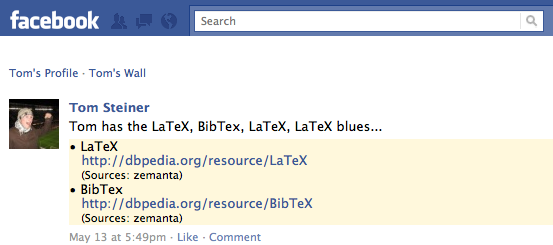
\includegraphics[width=0.45\textwidth]{facebook-swarm-nlp.png}
  \caption{Facebook Swarm NLP Chrome Extension. Extracted named entities have a pale yellow background.}     
  \label{fig:facebook}
\end{figure}

The remainder of this paper is structured as follows: In Section~\ref{sec:services}, we introduce two classes of Web
services that allow for unstructured data to be converted into Linked Data. In Section~\ref{sec:consolidation}, we
detail our entity consolidation approach with URI lookup and NLP Web services. In Section~\ref{sec:representing}, we
present how video annotations are represented in RDF. In Section~\ref{sec:tracking}, we describe how we automatically
maintain provenance metadata in our Web service. We discuss related work in Section~\ref{sec:related} and finally
conclude in Section~\ref{sec:conclusion}.

%%%%%%%%%%%%%%%%%%%%%%%%%%%%%%%%%%%%%%%%%%%%%%%%%%%%%%%%%%%%%%%%%%%%%%%%%%%
%%%  2. Web services for converting unstructured data into Linked Data  %%%
%%%%%%%%%%%%%%%%%%%%%%%%%%%%%%%%%%%%%%%%%%%%%%%%%%%%%%%%%%%%%%%%%%%%%%%%%%%

\section{Web services for converting unstructured data into Linked Data}    \label{sec:services}
In this section, we describe both Natural Language Processing (NLP) and URI lookup Web services.

%%%  2.1 NLP Web Services  %%%
\subsection{NLP Web Services}                                               \label{sec:nlp}
The NLP Web services that we use for our experiments take a text fragment as an input, perform Named Entity Recognition
(NER) on it and then link the extracted entities back into the Linked Open Data (LOD)
cloud\footnote{\url{http://lod-cloud.net/}}. We use
OpenCalais\footnote{\url{http://www.opencalais.com/documentation/}},
Zemanta\footnote{\url{http://developer.zemanta.com/docs/}} and
AlchemyAPI\footnote{\url{http://www.alchemyapi.com/api/entity/}} as NLP Web services.

% DVD: is there a reason that you not use the DBPedia SPARQL endpoint?
% TOM: See ref{sec:technicalnote}

%%%  2.2 URI Lookup Web Services  %%%
\subsection{URI Lookup Web Services}                                        \label{sec:urilookup}
The URI lookup Web services take a term as an input and return the set of URIs that most probably represent this term.
We use Freebase\footnote{\url{http://wiki.freebase.com/wiki/Search}}, DBpedia
Lookup\footnote{\url{http://lookup.dbpedia.org/}}, Sindice\footnote{\url{http://sindice.com/developers/api}}, and
Uberblic\footnote{\url{http://uberblic.org/developers/apis/search/}} as URI lookup Web services.

%%%  2.3 Technical Note  %%%
\subsection{Technical Note}                                                 \label{sec:technicalnote}
For both classes of services, we use them in parallel, aiming at the emergence effect in the sense of Aristotle:
``\emph{[\ldots] the totality is not, as it were, a mere heap, but the whole is something besides the parts
[\ldots]}''\footnote{Aristotle, Metaphysics, Book H 1045a 8-10.}. Our Web service is written in JavaScript and is based
on Node.js\footnote{\url{http://nodejs.org/}} and the Express\footnote{\url{http://expressjs.com/index.html}} framework.
As JSON and XML are well-supported by JavaScript, we use the third parties' JSON or XML APIs as a means of communication with all services, and not the
potential SPARQL endpoints or RDF APIs. In the next section, we describe our strategies for entity consolidation in
both cases.

%%%%%%%%%%%%%%%%%%%%%%%%%%%%%%%%%
%%%  3. Entity Consolidation  %%%
%%%%%%%%%%%%%%%%%%%%%%%%%%%%%%%%%

\section{Entity Consolidation}                                              \label{sec:consolidation}
We define the process of entity consolidation as the merge of entities, i.e., if several services extract the same
entity from the same input text fragment or term, we say that the entity is consolidated.

%%%  3.1 Interplay Of the Web Services  %%%
\subsection{Interplay Of the Web Services}                                  \label{sec:interplay}
As outlined before, the metadata for a YouTube video are its \textit{title}, its \textit{description}, its \textit{tags}, and its \textit{closed captions
tracks}. We first analyze the tags one-by-one with each URI lookup Web services through a helper wrapper sub-service of our Web service. We then
analyze the title combined with the description (first run) and the closed captions track (second run) through another wrapper helper sub-service with each of the NLP Web services. We have chosen this order because we have observed that sometimes video description
and closed captions are not related at all. This happens when the video description gets used not in a way to describe
the video content on a high level but, for example, to advertise different videos from the same user. In this case, the
NLP gets steered in a completely wrong direction. During our experiments, this occurred often enough for us to separate
the NLP analysis of descriptions and closed captions into two independent steps. When all these analysis steps are completed,
we try to match the extracted entities from all classes of services back in the video. In the following, we present our
approach for how to consolidate entities from URI lookup Web services and NLP Web services.

%%%  3.2 Entity Consolidation for URI Lookup Web Services  %%%
\subsection{Entity Consolidation for URI Lookup Web Services}               \label{sec:consolidation-uri}
As as first step, we have implemented a wrapper helper sub-service for all four URI lookup services (see~\ref{sec:urilookup}) that assimilates the particular
service's output to a common output format. This format is the least common multiple of the information of all Web
service results. For our experiments, we agreed on the JSON format. In the example below, we use the term ``Google
Translate'' to illustrate the approach. Three services return back a DBpedia URI, Sindice being the only one returning
a different result in a first place.
\begin{lstlisting}
[
  {
    "name": "Google Translate",
    "uris": [
      "http://dbpedia.org/resource/Google_Translate"
    ],
    "source": "freebase,uberblic,dbpedia",
    "relevance": 0.75
  }
]
\end{lstlisting}

The corresponding request to our wrapper API that calls all four URI lookup Web services in the background is via
\texttt{GET}
\url{/uri-lookup/combined/Google%20Translate} while the particular results from each service are available at
\url{/uri-lookup/{service_name}/Google%20Translate}.
We observe in this example that even in the lowest data representation level (JSON), we maintain provenance metadata in
the form of a \texttt{source} field.

In order to agree on a winner entity, a majority-based voting system is used. As soon as for two entities only one of
these entities' URIs match, we consider the entity consolidated and can merge the results. The problem, however, is
that both Freebase and Uberblic return results in their own namespaces (e.g., for ``Google Translate'' the results
are\nofootnote{\url{http://freebase.com/en/google_translate}},
and\nofootnote{\url{http://uberblic.org/resource/67dc7037-6ae9-406c-86ce-997b905badc8#thing}}), whereas Sindice and
DBpedia Lookup return results from DBpedia (Sindice returns other results as well). Freebase and Uberblic interlink
their results with DBpedia at an \url{owl:sameAs} level in the case of Freebase, and by referencing the source
(\url{umeta:source_uri}) for Uberblic. Therefore, by retrieving and parsing the referenced resources in the services'
namespaces, we can map back to DBpedia URIs and thus match all four services' results on the DBpedia level. Each
service's result contributes with a relevance of 0.25 to the final result. In this example, when three services agree
on the same result, the resulting relevance is thus the sum of the singular relevance scores (0.75 in this case).

%%%  3.3 Entitiy Consolidation for NLP Web Services  %%%
\subsection{Entitiy Consolidation for NLP Web Services}                     \label{sec:consolidation-nlp}
Similarly to URI lookup entity consolidation, we have implemented a second wrapper helper Web service for the three NLP services (see~\ref{sec:nlp}). While the
original calls to each particular NLP service are all HTTP \texttt{POST}-based, we have implemented the wrapper
\texttt{GET}- and \texttt{POST}-based. All NLP Web services return entities with their types and/or subtypes, names,
relevance, and URIs that link into the LOD cloud. The problem is that each service has implemented its own typing
system and providing mappings for all of them would be a relatively time-consuming task. However, as all services
provide links into the LOD cloud, the desired typing information can be pulled from there in a true Linked Data manner. The least common
multiple of the results for the query ``Google Translate'' is depicted below. For the sake of clarity, we just show one
entity with two URIs while the original result contained seven entities among which six were relevant and one was just
related.
\begin{lstlisting}
[
  {
    "name": "Google Translate",
    "relevance": 0.7128319999999999,
    "uris": [
      {
        "uri": "http://dbpedia.org/resource/Google_Translate",
        "source": "alchemyapi"
      },
      {
        "uri": "http://rdf.freebase.com/ns/en/google_translate",
        "source": "zemanta"
      }
    ],
    "source": "alchemyapi,zemanta"
  }
]
\end{lstlisting}

These results come from a request to our wrapper API via \texttt{GET} \url{/entity-extraction/combined/Google%20Translate},
and similarly to the URI lookup, the particular services' results can be obtained at \url{/entity-extraction/{service_name}/Google%20Translate%20is%20a%20service%20by%20Google}.
While AlchemyAPI and Zemanta return results from DBpedia and other interlinked LOD cloud resources, OpenCalais returns
only results in its own namespace
(e.g.\nofootnote{\url{http://d.opencalais.com/er/company/ralg-tr1r/ce181d44-1915-3387-83da-0dc4ec01c6da.rdf}} for the
company Google). In this particular case, retrieving the resource RDF representation and parsing for
\texttt{owl:sameAs} return links to DBpedia. However, in the general case, we found OpenCalais URIs sometimes pointing
to non-existent resources or to not very rich resources such
as\nofootnote{\url{http://d.opencalais.com/pershash-1/cfcf1aa2-de05-3939-a7d5-10c9c7b3e87b.html}}, a URI identifying
the current US President Barack Obama where the only information is that Barack Obama is of type person. In order to
consolidate extracted entities, we use the following approach: we have a look at each of the extracted entities from
service one and compare each entity's URIs with each URIs from each extracted entity from service two. The examples
below illustrate this process.

First, we consider the isolated results for the text fragment from AlchemyAPI only:
\begin{lstlisting}
{
  "name": "Google",
  "relevance": 0.496061,
  "uris": [
    {
      "uri": "http://dbpedia.org/resource/Google",
      "source": "alchemyapi"
    },
    {
      "uri": "http://rdf.freebase.com/ns/guid.9202a8c04000641f800000000042acea",
      "source": "alchemyapi"
    },
    {
      "uri": "http://cb.semsol.org/company/google.rdf",
      "source": "alchemyapi"
    }
  ],
  "source": "alchemyapi"
}
\end{lstlisting}

Second, we consider the isolated results for the same text fragment from Zemanta only:
\begin{lstlisting}
{
  "name": "Google Inc.",
  "relevance": 0.563132,
  "uris": [
    {
      "uri": "http://rdf.freebase.com/ns/en/google",
      "source": "zemanta"
    },
    {
      "uri": "http://dbpedia.org/resource/Google",
      "source": "zemanta"
    },
    {
      "uri": "http://cb.semsol.org/company/google#self",
      "source": "zemanta"
    }
  ],
  "source": "zemanta"
}
\end{lstlisting}

Finally, we consider the merged results from both Zemanta and AlchemyAPI. Note that these results are not exposed externally, they are used internally by the wrapper helper Web service:
\begin{lstlisting}
{
  "name": [
    "Google",
    "Google Inc."
  ],
  "relevance":  0.5295965,
  "uris": [
    {
      "uri": "http://dbpedia.org/resource/Google",
      "source": "alchemyapi"
    },
    {
      "uri": "http://rdf.freebase.com/ns/guid.9202a8c04000641f800000000042acea",
      "source": "alchemyapi"
    },
    {
      "uri": "http://umbel.org/umbel/ne/wikipedia/Google",
      "source": "alchemyapi"
    },
    {
      "uri": "http://cb.semsol.org/company/google.rdf",
      "source": "alchemyapi"
    },
    {
      "uri": "http://rdf.freebase.com/ns/en/google",
      "source": "zemanta"
    },
    {
      "uri": "http://cb.semsol.org/company/google#self",
      "source": "zemanta"
    }
  ],
  "source": "alchemyapi,zemanta"
}
\end{lstlisting}

In this example, the entity names mismatch (``google inc.'' vs. ``google''). However, going down the list of URIs for
the entity, one can note a match via\nofootnote{\url{http://dbpedia.org/resource/Google}}. Additionally, one can also
see two would-be matches: \nofootnote{\url{http://cb.semsol.org/company/google.rdf}}
vs.\nofootnote{\url{http://cb.semsol.org/company/google#self}} and
\nofootnote{\url{http://rdf.freebase.com/ns/en/google}} vs.
\nofootnote{\url{http://rdf.freebase.com/ns/guid.9202a8c04000641f800000000042acea}}. However, the inconsistent use of
URIs when there is more than one URI available for the same entity hinders the match from being made. An additional
retrieval of the resources would be necessary to detect that in the latter case
\nofootnote{\url{http://rdf.freebase.com/ns/guid.9202a8c04000641f800000000042acea}} redirects to
\nofootnote{\url{http://rdf.freebase.com/ns/en/google}}, whereas the first example seems to be broken
(\nofootnote{\url{http://cb.semsol.org/company/google#self}} returns the status code 404). The good thing, however, is
that as soon as one match has been detected, one can consolidate the entities from both services.

Given the mismatching two entity names (``google inc.'' vs. ``google''), the consolidated name is then an array of all
detected synonymous. The consolidated relevance is the average relevance of both services. In contrast to URI lookup
where we had to manually assign a relevance of 0.25 to each result since not all URI lookup services include the
concept of relevance in their results, with NLP services, each service already includes a relevance score ranging from
0 (irrelevant) to 1 (relevant), so we can directly use it. In our approach, the consolidated and merged entities from
service one and two are then in turn compared to extracted entities from service three and so on, if we used even more
services. In practice, however, due to the not always given interconnectedness of OpenCalais, there are no matches
after having compared Zemanta-extracted entities with AlchemyAPI-extracted entities. Similarly to URI lookup-detected
entity consolidation, we also maintain provenance metadata for each URI on the lowest data representation level (JSON)
on both a per URI basis and an entity basis with the NLP-detected entity consolidation.

We note that in our example, the results from URI lookup are a subset of the results from NLP. However, while all URI
Lookup services accept one-word arguments (e.g., ``google''), only AlchemyAPI from the NLP services accepts one-word
arguments. The two other services accept only non-trivial text fragments (e.g., ``google is a company founded by larry
page'').

%%%  3.4 Identity Links On the Semantic Web  %%%
\subsection{Identity Links On the Semantic Web}                             \label{sec:sameasorg}
In order to tackle the problem of different namespaces in results that we have outlined in the
Section~\ref{sec:consolidation-uri}, a straightforward idea is to use a Web service such as
<sameAs>\footnote{\url{http://sameas.org/}} to easily find mappings from one namespace into another. In practice,
however, while many data sources in the Linked Data world are marked as being equal to each other (e.g.,
\url{http://dbpedia.org/resource/Barack_Obama} \texttt{owl:sameAs} \url{http://rdf.freebase.com/rdf/en.barack_obama}),
the quality of such equality links is not always excellent. As Halpin et al. show in~\cite{Halpin:SameAs}, the problem
with \texttt{owl:sameAs} is that people tend to use it very differently. The authors of~\cite{Halpin:SameAs}
differentiate four separate usage styles, each with its particular implications. Inference is thus problematic, if not
impossible, when the sense of the particular use of \texttt{owl:sameAs} is unknown.

%%%  3.5 Design of the Web Service  %%%
\subsection{Design of the Web Service}                                      \label{sec:design}
% DVD: will you publish the URI where we and reviewers can test the web service?
% TOM: As all this stuff is Node-based, I could not find an external hosting service yet (I signed up for Heroku and Joyent, but am still on the waiting list and I'm not sure if they will allow me to do all what I want to do). So short, it's localhost for the moment. Plus the code is not really rock-solid yet, but it works.

Our Web service is designed with RESTful design principles in mind: properly named resources, use of the adequate HTTP
verbs, and implementation of Hypermedia Controls (also known as
HATEOAS\footnote{\url{http://martinfowler.com/articles/richardsonMaturityModel.html#level3}}). Currently, the Web
service supports the following operations:
\begin{itemize}
\item Looking up URIs for a given term (allowed service names are ``dbpedia", ``freebase", ``uberblic", ``sindice", and ``combined"): \texttt{GET} \url{/uri-lookup/{service_name}/{term}}
\item Extracting entities from a given text fragment (allowed service names are ``opencalais", ``zemanta", ``alchemyapi", and ``combined"): \texttt{GET} | \texttt{POST} \url{/entity-extraction/{service_name}/{text_fragment}}\footnote{In the case of \texttt{POST}, the \texttt{\{text\_fragment\}} has to be sent in the body of the HTTP message.}
\item Getting an RDF annotation for a video with a given video ID: \texttt{GET} \url{/youtube/rdf/{video_id}}
\item Modifying or manually creating an RDF annotation for a video with a given video ID: \texttt{PUT} \url{/youtube/rdf/{video_id}}
\item Deleting an RDF annotation for a video with a given video ID: \texttt{DELETE} \url{/youtube/rdf/{video_id}}
\item Getting metadata from YouTube for a video with a given video ID: \texttt{GET} \url{/youtube/video/{video_id}}
\item Getting all closed captions from YouTube for a video with a given video ID: \texttt{GET} \url{/youtube/video/{video_id}/closedcaptions}
\item Getting closed captions in a given language from YouTube for a video with a given video ID: \texttt{GET} \url{/youtube/video/{video_id}/closedcaptions/{language_code}}
\item Getting a plain text audio transcription from YouTube for a video with a given video ID: \texttt{GET} \url{/youtube/video/{video_id}/audiotranscription}
\item Getting a plain text audio transcription in a given language from YouTube for a video with a given video ID: \texttt{GET} \url{/youtube/video/{video_id}/audiotranscription/{language_code}}
\end{itemize}

%%%%%%%%%%%%%%%%%%%%%%%%%%%%%%%%%%%%%
%%%  4. Describing Videos in RDF  %%%
%%%%%%%%%%%%%%%%%%%%%%%%%%%%%%%%%%%%%

\section{Describing Videos in RDF}                                          \label{sec:representing}
In this section, we present the particular components of the video metadata available and their representation in RDF.

%%%  4.1 Basic YouTube Metadata  %%%
\subsection{Basic YouTube Metadata}                                         \label{sec:metadata}
We use the W3C Ontology for Media Resources~\cite{W3C:MediaOntology} as the central vocabulary, mainly because it
already defines a set of
mappings\footnote{\url{http://www.w3.org/2008/WebVideo/Annotations/drafts/ontology10/CR/test.php?table=YouTube}} not
only for YouTube metadata, but also for many other existing metadata formats. This ontology aims to foster the
interoperability among various kinds of metadata formats currently used to describe media resources on the Web. From
this vocabulary, we use the following properties: \url{ma:title}, \url{ma:creator}, \url{ma:createDate},
\url{ma:description} and others technical properties which have direct mappings to YouTube metadata.

%%%  4.2 YouTube Tags  %%%
\subsection{YouTube Tags}                                                   \label{sec:youtube}
In order to represent YouTube tags, or rather, semantically annotated YouTube tags, we use the Common Tag
vocabulary~\cite{CommonTag:Spec}. A resource is \url{ctag:tagged} with a \url{ctag:Tag} which consists of a textual
\url{ctag:label} and a pointer to a resource that specifies what the label \url{ctag:means}. The Common Tag vocabulary
is well-established and developed by both industry and academic partners.

%%%  4.3 Entities in Video Fragments  %%%
\subsection{Entities in Video Fragments}
As stated before, the current video annotation Web service is a re-implementation of our previous client-side
application SemWebVid~\cite{Steiner:SemWebVid}. Hence, we already could collect some experience with modeling video
data in RDF on our own, and were also inspired by the semantic video search engine
yovisto\footnote{\url{http://yovisto.com/}}~\cite{Sack:Use,Sack:VideoSearch}. In our first attempt, we used the Event
Ontology\cite{Raimond:Event} and defined each line (which not necessarily corresponds to a complete sentence) in the
closed captions track as an \url{event:Event}. In the current implementation, we simplified the annotation model by
removing the notion of events, and by introducing the notion of video fragments instead. We split the single lines in
the complete closed captions track in complete sentences. Consequently, a video fragment now stretches over a complete
sentence which usually contains more than just one line in the closed captions track. This matches much more the human
perception of a self-contained incident in a video.

For addressing a video fragment, we use the Media Fragment URIs~\cite{W3C:MediaFrags} specification. Media Fragment
URIs are also supported by the Ontology for Media Resources via the \url{ma:MediaFragment} property. In particular, we
use the temporal dimension (e.g.\nofootnote{\url{http://example.org/video.webm#t=10,20}}) which is defined by its start
and end time relative to the entire video play time. In addition to the temporal dimension, we also use the track
dimension (e.g.\nofootnote{\url{http://example.org/video.webm#track=closedcaptions}}) which allows for addressing only
a closed captions track. The value of the parameter \texttt{track} is a free-form UTF-8 string, so we are flexible with
regards to its usage.

In the previous SemWebVid implementation, we used \url{event:factor}, \url{event:product}, and \url{event:agent} to
relate events with factors (non-person entities extracted), products (particular plain text closed captions lines), and
agents (persons extracted). In the current implementation, we consistently use the same Common Tag vocabulary to
annotate entities in a temporal video fragment (see Section~\ref{sec:youtube}). We thus have:
\begin{lstlisting}
<http://example.org/video.webm#t=10,20>
  a ma:MediaFragment ;
  ctag:tagged
    [ a ctag:Tag ;
      ctag:label "example" ;
      ctag:means <http://example.org/example#>
    ] .
\end{lstlisting}

%%%%%%%%%%%%%%%%%%%%%%%%%%%%%%%%%%%%%%%%%%%%%%%%%%%%%%%%%%%
%%%  5. Tracking Provenance With Multiple Data Sources  %%%
%%%%%%%%%%%%%%%%%%%%%%%%%%%%%%%%%%%%%%%%%%%%%%%%%%%%%%%%%%%

\section{Tracking Provenance With Multiple Data Sources}                    \label{sec:tracking}
As outlined before, we use several data sources (Web services) in the background in order to deploy our own video annotation Web service.
The simple example fact produced by our service that a \url{ma:MediaFragment} is \url{ctag:tagged} with a \url{ctag:Tag}
with the \url{ctag:label} ``\url{label}", where what this \url{ctag:label} \url{ctag:means} is
represented by an example entity with the URI \url{http://example.org/example#}, might in consequence have been the
result of up to seven agreeing (or disagreeing) Web service calls. In order to track the contributions of the various
sources, we decided to use the Provenance Vocabulary~\cite{Hartig:Provenance} by Hartig and Zhao with the prefix \texttt{prv}, and the HTTP Vocabulary in RDF~\cite{HTTP:RDF} by Koch et al. with prefix \texttt{http}. We chose the HTTP Vocabulary in RDF for the fact that it is a W3C Working Draft  developed by the Evaluation and Repair Tools Working Group (ERT WG), which is part of the World Wide Web Consortium (W3C) Web Accessibility Initiative (WAI). The Provenance Vocabulary was chosen because of its relatively broad implementation in several projects, such as Pubby\footnote{\url{http://www4.wiwiss.fu-berlin.de/pubby/}}, Triplify\footnote{\url{http://triplify.org/Overview}}, and D2R Server\footnote{\url{http://www4.wiwiss.fu-berlin.de/bizer/d2r-server/}}.

We are driven by the motivation that even if the direct
requests of our Web service were made against two wrappers (see Section~\ref{sec:consolidation-uri} and
Section~\ref{sec:consolidation-nlp}), we still want to be able to credit back the results to the original calls to the third party
Web services.

We have two basic cases that affect the RDF describing the data provenance: requests per HTTP \texttt{GET} and requests
per HTTP \texttt{POST}. All URI lookup services that we use are \texttt{GET}-based. All of our NLP services are
\texttt{POST}-based. In order to make statements about a bundle of triples, we group them in a named graph. We use the
TriG~\cite{Bizer:TriG} syntax:
\begin{lstlisting}
:G = {
  <http://example.org/video.webm#t=10,20>
    a ma:MediaFragment ;
    ctag:tagged [
      a ctag:Tag ;
      ctag:label "label" ;
      ctag:means <http://example.org/example#>
    ] .
} .
\end{lstlisting}

%%%  5.1 The Provenance Vocabulary  %%%
\subsection{The Provenance Vocabulary}                                      \label{sec:provenance}
In this section, we outline the required steps in order to make statements about the provenance of a group of triples
contained in a named graph \url{:G} that was generated using several HTTP \texttt{GET} requests to third party Web
services. We use the Provenance Vocabulary~\cite{Hartig:Provenance} with the prefix \texttt{prv} and the HTTP Vocabulary in RDF~\cite{HTTP:RDF} with prefix \texttt{http}. The text below can be best followed by looking at the triples in the next section~\ref{sec:appendix}.

First, we state that \url{:G} is both a \url{prv:DataItem} and obviously an \url{rdfg:Graph}. \url{:G} is
\url{prv:createdBy} the process of a \url{prv:DataCreation}. This \url{prv:DataCreation} is \url{prv:performedBy} a
\url{prv:NonHumanActor}, a \url{prvTypes:DataCreatingService} to be precise. This service is \url{prv:operatedBy} a
human (\url{http://tomayac.com/thomas_steiner.rdf#me}). Time is often important for provenance, so the
\url{prv:performedAt} date of the \url{prv:DataCreation} needs to be saved. During the process of the
\url{prv:DataCreation} there are \url{prv:usedData}, which are \url{prv:retrievedBy} a \url{prv:DataAcess} that is
\url{prv:performedAt} a certain time, and \url{prv:performedBy} a non-human actor (our Web service) that is
\url{prv:operatedBy} a human (\url{http://tomayac.com/thomas_steiner.rdf#me}. For the \url{prv:DataAccess} (there is
one for each third party Web service involved), we \url{prv:accessedService} from a \url{prv:DataProvidingService} of
which we \url{prv:accessedResource} at a certain \url{irw:WebResource}. Therefore, we
\url{prvTypes:exchangedHTTPMessage} which is an \url{http:Request} using \url{http:httpVersion} ``1.1'' and the
\url{http:methodName} ``GET''.

\subsection{Provenance RDF Overview}                                           \label{sec:appendix}
This section provides a shortened overview of the provenance RDF in Turtle syntax for a YouTube tag with the label ``obama'' and the assigned
meaning \url{http://dbpedia.org/resource/Barack_Obama} (for the sake of brevity, only two of the \url{prv:usedData}
sources are mentioned, namely Freebase and DBpedia Lookup). The named graph \url{:G} in the first part of the listing contains the absolute data (the fact that the YouTube video with the ID ``3PuHGKnboNY" is tagged with the label ``obama", which means Obama in the sense of \url{http://dbpedia.org/resource/Barack_Obama}). The second part with metadata about \url{:G} basically says that these facts were generated via two calls: \url{http://api.freebase.com/api/service/search?format=json&query=obama} and \url{http://lookup.dbpedia.org/api/search.asmx/KeywordSearch?QueryString=obama}:
\begin{lstlisting}
:G = {
  <http://gdata.youtube.com/feeds/api/videos/3PuHGKnboNY> ctag:tagged :tag .
  :tag
    a ctag:Tag ;
    ctag:label "obama" ;
    ctag:means <http://dbpedia.org/resource/Barack_Obama> ;
} .


:G
  a prv:DataItem ;
  a rdfg:Graph ;
  prv:createdBy [
    a prv:DataCreation ;
    prv:performedAt "2011-05-01T12:42:30Z"^^xsd:dateTime ;
    prv:performedBy [
      a prv:NonHumanActor ;
      a prvTypes:DataCreatingService ;
      prv:operatedBy <http://tomayac.com/thomas_steiner.rdf#me> .
    ] ;
    prv:usedData [
      prv:retrievedBy [
        a prv:DataAcess ;
        prv:performedAt "2011-05-01T12:42:30Z"^^xsd:dateTime ;
        prv:performedBy [
          prv:operatedBy <http://tomayac.com/thomas_steiner.rdf#me> .
        ] ;
        prv:accessedService <http://api.freebase.com/api/service/search> ;
        prv:accessedResource <http://api.freebase.com/api/service/search?format=json&query=obama> ;
        prvTypes:exchangedHTTPMessage [
          a http:Request ;
          http:httpVersion "1.1" ;
          http:methodName "GET" ;
          http:mthd <http://www.w3.org/2008/http-methods#GET> ;
          http:headers (
            [
              http:fieldName "Host" ;
              http:fieldValue "api.freebase.com" ;
              http:hdrName <http://www.w3.org/2008/http-header#host> ;
            ]
          )
        ] ;
      ] ;
    ] ;
    prv:usedData [
      prv:retrievedBy [
        a prv:DataAcess ;
        prv:performedAt "2011-05-01T12:42:30Z"^^xsd:dateTime ;
        prv:performedBy [
          prv:operatedBy <http://tomayac.com/thomas_steiner.rdf#me> .
        ] ;
        prv:accessedService <http://lookup.dbpedia.org/> ;
        prv:accessedResource <http://lookup.dbpedia.org/api/search.asmx/KeywordSearch?QueryString=obama> ;
        prvTypes:exchangedHTTPMessage [
          a http:Request ;
          http:httpVersion "1.1" ;
          http:methodName "GET" ;
          http:mthd <http://www.w3.org/2008/http-methods#GET> ;
          http:headers (
            [
              http:fieldName "Host" ;
              http:fieldValue "lookup.dbpedia.org" ;
              http:hdrName <http://www.w3.org/2008/http-header#host> ;
            ]
          )
        ] ;
      ] ;
    ] ;
  ] .
} .
\end{lstlisting}

%%%  5.2 Tracking Provenance With Human Interaction  %%%
\subsection{Tracking Provenance With Human Interaction}                     \label{sec:human}
RDF video annotations that are completely automatically generated often need to be manually corrected. In our RESTful
Web service, we have thus envisioned that not only a big archive of automatically generated video annotations gets
built, but that also people can correct errors (via HTTP \texttt{PUT} or later \texttt{PATCH}) in the RDF interactively
(or remove completely wrong video annotations via HTTP \texttt{DELETE}). For the correction case, this can be tracked
using the Provenance Vocabulary as follows. Let us assume we wanted to replace an unfriendly Freebase \url{ctag:means}
resource of\nofootnote{\url{http://rdf.freebase.com/ns/guid.9202a8c04000641f800000000042acea}} with the friendlier
variant\nofootnote{\url{http://rdf.freebase.com/rdf/en.google}}:
\begin{lstlisting}
:G_corrected = {
  <http://gdata.youtube.com/feeds/api/videos/3PuHGKnboNY>
  ctag:tagged [
    a ctag:Tag ;
    ctag:label "google" ;
    ctag:means <http://rdf.freebase.com/rdf/en.google>
  ]
} .
:G_corrected
  a prv:DataItem ;
  a rdfg:Graph ;
  prv:createdBy [
    a prv:DataCreation ;
    prv:performedAt "2011-05-01T12:42:30Z"^^xsd:dateTime ;
    prv:performedBy [
      a prv:HumanActor ;
      <http://tomayac.com/thomas_steiner.rdf#me>
    ]
  ] .
\end{lstlisting}

The \url{prv:DataCreation} no longer contains references to \url{prv:usedData}. Obviously, this approach to identify a
\url{prv:HumanActor} with a FOAF profile requires an authentication step which might not always be desired. One could
think of a ``John Doe''-like anonymous pseudo-\url{prv:HumanActor}, or in the case of an intendedly non-anonymous
\url{prv:HumanActor}, authentication methods like WebID\footnote{\url{http://www.w3.org/2005/Incubator/webid/charter}}
could be used.

%%%  5.3 The Need for Providing Provenance Metadata  %%%
\subsection{The Need for Providing Provenance Metadata}
Hartig et al. mention in~\cite{ipaw10:olaf} some reasons that justify the need for provenance metadata. Among those,
linked dataset replication and distribution on the Web with not necessarily always the same namespaces: based on the
same source data, different copies of a linked dataset can be created with different degrees of interconnectedness by
different publishers.

We add to this list the automatic conversion of legacy unstructured data to Linked Data with heuristics where extracted
entities -- while being consolidated and backed up by different data sources -- might still be wrong. Especially with our
``mash-up''-like approach, it is very desirable to be able to track back to the concrete source where a certain piece
of information might have come from. This enables a) to correct the error at the root of our Web service (fighting the
cause), b) to correct the concrete error in an RDF annotation (fighting the symptom), or c) to judge the
trustworthiness and quality of a dataset which is probably the most important reason.

%%%  5.4 Change Of Referenced Datasets Over Time  %%%
\subsection{Change Of Referenced Datasets Over Time}                        \label{sec:change}
It is to be noted that a statement such as the triple below refers to the triple object as an identifier for a Web
resource (where the Web resource is a representation of the result of the API call at the time where it was
\url{prv:performedAt}).
\begin{lstlisting}
_:x prv:accessedResource <http://api.freebase.com/api/service/search?format=json&query=obama> ;
\end{lstlisting}
As provenance metadata always refer to the time context in which a certain statement was made, it is essentially
unimportant what representation the resource returns at a later time.

%%%%%%%%%%%%%%%%%%%%%%%%%%%%%%%%%%%%
%%%  6. Related And Future Work  %%%
%%%%%%%%%%%%%%%%%%%%%%%%%%%%%%%%%%%%

\section{Related Work}\label{sec:related}
Given the concrete use case of our approach, we decided to split up this section in two parts. First, related work in the field of mash-up Web service provenance, and second, related work in the field of semantic video description.

\subsection{Mash-up Web Service Provenance Related Work}
In~\cite{Groth:2009:MPD:1462159.1462162}, Groth et al. describe how through tools and technologies such as Yahoo Pipes, Really Simple Syndication (RSS) and Web services, so-called mash-ups can be created in a dynamic, just-in-time way, combining data from different data sources. The authors are driven by the motivation to allow for trust and confidence in mash-ups, and therefore (just like us) consider it critical to be able to analyze the origin of combined results. They suggest an approach based on OWL and XML, with a focus on process documentation. However, different from us, where the goal is to transparently add provenance data at Web service invocation level, there focus is more on overall process documentation in the context of a mash-up application.

The focus of Carroll et al. in~\cite{carroll2005} is on the provenance of triples in the Semantic Web world, namely, for making statements about triples in graphs, therefore the paper introduces the concept of named graphs, an extension to RDF. In contrast to our work, Carroll et al. focus purely on using triples to make statements about triples (that is, they stay in the RDF world), whereas our approach uses RDF to make statements about potentially any Web service result, albeit in the mentioned concrete case, we use RDF as such Web service result. It is to be noted, however, that our approach is not limited to RDF results.

In the WS-* world, BPEL4WS, described by Curbera et al. in~\cite{Curbera:2003:NSW:944217.944234} provides a formal language for the specification of business processes and business interaction protocols. This allows for the combination of several Web services, however, does not credit back concrete outputs of a combined Web service to the underlying Web services.

\subsection{Video Description Related Work}

In~\cite{Sack:VideoSearch}, Waitelonis et al. address the problem of how to deploy exploratory search for video data by
using semantic search technology for the yovisto video search engine. They show how exploratory search can be enriched
by information from the LOD cloud in order to facilitate navigation in big video archives. Yovisto supports several
ways to annotate a video with metadata: video-related, and video-time-related tags. Video-related tags are applied to
the entire video and are entered by the initial video uploader, whereas video-time-related tags only apply to a certain
point in the video. They can either be automatically extracted from the video on a certain timestamp (e.g. by analyzing
the video images with OCR methods), or can be user-generated tags also on a certain timestamp. In a different paper,
Waitelonis et al. show how using permutations of a term and this term's surrounding context and by detecting paths
between entities, a legacy keyword-based video search engine can be converted into a semantic video search
engine~\cite{Sack:Use}. This approach uses a keyword-to-DBpedia-URI mapping heuristic. However, as far as we can tell,
provenance metadata is not maintained. Future work will compare the results of the yovisto heuristic with ours using
agreed-on benchmarks.

In~\cite{Choudhury:YouTube}, Choudhury et al. describe a framework for semantic enrichment, ranking, and integration of
Web video tags using Semantic Web technologies. In order to enrich the user-generated tag space which is often sparse,
metadata such as the recording time and location, the video title and video description, social features such as
playlists that a video appears in and related videos, etc. are used. Next, the tags are ranked by their co-occurrence
and in a final step interlinked to DBpedia concepts for greater integration with other datasets. Choudhury et al.
disambiguate the tags using WordNet\footnote{\url{http://wordnet.princeton.edu/}} synsets if possible. This means that
if there is only one matching synset in WordNet, the corresponding WordNet URI in DBpedia is selected. If there are
more than one matching synsets, the tags and their context tags similarity are computed and thereby tried to decide on
an already existing tag URI. For words that are not contained in WordNet, Sindice is used to find the most probable
concept. To the best of our knowledge provenance metadata is not maintained.

%%%%%%%%%%%%%%%%%%%%%%%
%%%  7. Conclusion  %%%
%%%%%%%%%%%%%%%%%%%%%%%

\section{Conclusion}                                                        \label{sec:conclusion}
We have introduced a Web service for semantic text-based video annotation for YouTube videos with closed captions. As mash-up data sources for our Web service, we have
presented several URI lookup and NLP Web services and showed our approach for both classes of Web services to
consolidate entities. We then focused on the necessary RDF vocabularies and Media Fragment URIs to annotate
video-related and video-time-related entities. Due to their different ``mash-up''-like history of origins, we need to
track provenance metadata in order to assure the trustworthiness of the generated data. We showed how the Provenance
Vocabulary can be used to keep track of the original third party Web service calls that led to the consolidated
results. These references to the original calls are to be understood as the identificator of Web resources (i.e. the
results of a request). We have shown how a concrete multi-source RESTful Web service can automatically maintain provenance
metadata, both for entirely machine-generated content, but also for partly (or completely) human-generated content. We
believe that being able to track back the origin of a triple is of crucial importance, especially given the network
effect which is one of the Linked Data benefits. The generated triples are very verbose, and in consequence stating even simple facts that a combined result is based on two separate sub-results takes up a lot of space. The verbosity is mainly due to the used vocabularies, the Provenance Vocabulary and the HTTP Vocabulary in RDF.

Already commenced future work will be to explore ways to stick to existing standards as these vocabularies on the one hand, but on the other hand to simplify drastically in order to come to less verbose provenance descriptions. While it is always easier to come up with a specialized vocabulary that does one task well (for example we could imagine a simple vocabulary with the sole purpose to log the API call of a Web service invocation), broader reuse and acceptance can be gained by reusing existing vocabularies. We will see how to find the right balance here, and are conscious that our current approach is a first step in that direction, however, that many more steps are ahead to take. Our vision is to establish a common method for specifying provenance data for mash-up Web services. 

% conference papers do not normally have an appendix

% use section* for acknowledgement
\section*{Acknowledgment}

We would like to thank Olaf Hartig from the Humboldt-Universit\"{a}t zu Berlin for his kind support with the correct
use of the Provenance Vocabulary. This work was partly supported by the European Commission under Grant No. 248296 FP7
I-SEARCH project and by the French Ministry of Industry (\emph{Innovative Web} call) under contract 09.2.93.0966,
``Collaborative Annotation for Video Accessibility'' (ACAV).


% trigger a \newpage just before the given reference
% number - used to balance the columns on the last page
% adjust value as needed - may need to be readjusted if
% the document is modified later
%\IEEEtriggeratref{8}
% The "triggered" command can be changed if desired:
%\IEEEtriggercmd{\enlargethispage{-5in}}

% references section

% can use a bibliography generated by BibTeX as a .bbl file
% BibTeX documentation can be easily obtained at:
% http://www.ctan.org/tex-archive/biblio/bibtex/contrib/doc/
% The IEEEtran BibTeX style support page is at:
% http://www.michaelshell.org/tex/ieeetran/bibtex/
%\bibliographystyle{IEEEtran}
% argument is your BibTeX string definitions and bibliography database(s)
%\bibliography{IEEEabrv,../bib/paper}
%
% <OR> manually copy in the resultant .bbl file
% set second argument of \begin to the number of references
% (used to reserve space for the reference number labels box)
\bibliographystyle{abbrv}
\bibliography{nwesp2011}

% that's all folks
\end{document}


